
% Author: PokMan Ho pok.ho19@imperial.ac.uk
% Script: LogisticTmp.tex
% Desc: `LaTex` report framework -- Logistic Growth
% Input: none
% Output: none
% Arguments: 0
% Date: Oct 2019

\documentclass[a4paper, 11pt]{article}
\usepackage[margin=1in]{geometry}
\usepackage{hyperref, setspace, lineno, amsmath, amssymb, longtable}
\usepackage{float} %% fix graphs at where they should be

%% test insert graphs
\usepackage{graphicx}
\graphicspath{ {../results/} } %% <https://www.overleaf.com/learn/latex/Inserting_Images>

%% test insert variables
\newcommand{\pml}{phenological model}
\newcommand{\pms}{phenological models}
\newcommand{\Pml}{Phenological model}
\newcommand{\Pms}{Phenological models}
\newcommand{\ReportTitle}{Microbial growth models -- which is better and why?} %% <https://stackoverflow.com/questions/1211888/is-there-any-way-i-can-define-a-variable-in-latex>
\newcommand{\ReportAuthor}{PokMan HO}
\newcommand{\ReportAffil}{Department of Life Sciences, Faculty of Natural Sciences,\\Imperial College London}
\newcommand{\Disclaim}{\textbf{A Mini-project submitted in partial fulfilment of the requirements for the degree of Master of Research at Imperial College London\\\\Formatted in the journal style of the \textit{Nature} Journal\\Submitted for the MRes in Computational Methods of Ecology and Evolution}}
\newcommand{\fve}{Verhulst (classical)}
\newcommand{\fgo}{modified Gompertz}
\newcommand{\fba}{Baranyi}
\newcommand{\fbu}{Buchanan}
\newcommand{\fqu}{quadratic}
\newcommand{\fcu}{cubic}
\newcommand{\pop}{population size}
\newcommand{\pps}{population sizes}

\title{\ReportTitle}
\author{\ReportAuthor\ (CID: 01786076)}
\date{}

%% citation
\usepackage[%
autocite    = superscript,
backend     = bibtex,
sortcites   = true,
style       = nature
]{biblatex}
\bibliography{../reference/Log_r.bib} %% <https://tex.stackexchange.com/questions/6805/bib-library-file-in-a-different-directory-how-to-use-mendeley-centralised-b>

%% set as required
\doublespacing
\linenumbers

\begin{document}
	\begin{center}
		\Huge\textbf{\ReportTitle}\\
		\LARGE\ReportAuthor\\
		\Large\ReportAffil
	\end{center}
	\begin{figure}[h]
		\centering
\includegraphics[width=\linewidth]{icl.jpg}
	\end{figure}
	\begin{flushright}
		\Large Approximate Word Count: %% insert approx word count
	\end{flushright}
	\clearpage
	
	\maketitle
	\section*{Abstract}
	\Pms\ have different features, assumptions and explanatory uses.  Hence choosing the correct and fittest model for your experimental data is crucial.  This project has used published microbial \pps\ data from ten papers to do non-parametric categorical analyses (i.e. Kruskal tests) and parameter evaluations (with PCA).  The result shows that \fve\ and \fgo\ are general models while \fba\ and \fbu\ are specific ones.  They have unobservable yet statistical differences in parameter responses.  Although \pms\ are not significantly better than polynomials on data descriptions, choosing the right model can potentially help discussing the data properties in microbial population of interest.
	
	\section*{Introduction}
	\Pms\ for microbial growth are expected to fit microbial population data.  Yet due to different reasons, models developed and published from one sample may not fit the others.  These reasons can be data variabilities, confounding factors, inaccurate assumptions or models being too-specific.  This data-mining project is aimed at comparing and contrasting published \pms\ on microbial \pop\ data, highlighting which is a better model under what conditions.  The hypotheses are:
	\begin{itemize}
		\item published \pms\ are significantly better fits than polynomials for describing microbial growths;
		\item appropriate \pml(s) is/are identifiable through distinguishable microbial \pop\ parameter values; and
		\item parameter values of each \pml\ from successful fits are clusters with well-defined boundaries between models.
	\end{itemize}
	Also, two biological hypotheses will be put forward:
	\begin{itemize}
		\item Microbial species combine with growth media is correlate with the AIC-optimal model (i.e. meeting the ``minimal AIC +2"\autocite{burnham2004multimodel} criteria); and
		\item Microbial species combine with growth media has its own parameter range for the optimal \pms.
	\end{itemize}
	
	\section*{Methods}
	
	Microbial \pps\ data were given, sourced from ten different publications (Table\ref{table:source}).  The collection contained different microbial clades growing at various conditions for varying times.  Also, these data were recorded in multiple time and population units.  Some of the population data were direct counts while some were not.
	
	Experimental microbial population growth data library were divided into individual data subsets through six filters (``Temperature (in $^o$C)", ``Microbial clade", ``growth substrate materials", ``experimental replicate number", ``population data recording unit" and ``data source").  Records with data unit ``OD\_595" were scaled into optical density percentages (i.e. data*100) to facilitate general analyses workflow.  Independent (or explanatory) variable was ``Time (hr)" and dependent (or response) variable was ``\pop".
	
	Some raw data were recorded in minutes (instead of hour).  This record artifact was not corrected because of two reasons: 1. shape of curves were the main concern instead of independent variable's scale; and 2. the unit was consistent within each data subset.
	
	\subsection*{Model assessment}
	Six candidate models were assessed, four phenological and two polynomial equations.  They were ``\fve"\autocite{mckendrick1912xlv}, ``\fgo"\autocite{GIL200689}, ``\fba"\autocite{baranyi1993modeling}, ``\fbu"\autocite{buchanan1993differentiation}, ``\fqu" and ``\fcu". Non-linear least square (NLLS) method was used only on the four \pms\ and linear approach was taken for the two polynomials.  Starting values selection (\pms\ only) was described below:
	
	Initial (N0) and final (K) \pps\ were selected to be the minimum and maximum values of each data subset respectively.  Maximum growth rate (r.max) and relative time lag (t.lag) were obtained through recursive linear modelling with shrinking independent range (from both maximum and minimum).  In this project 5\% was chosen as the shrinking threshold assuming this resolution was sufficient for initiating NLLS fits.  The final slope value (i.e. r.max) would be a positive finite number with the highest R$^{2}$ value (i.e. best-fit slope on considered data).  The x-intercept for that slope was the t.lag.  Time which this r.max linear model intersected with K was regarded as the time achieving carrying capacity (t.K).  Population data was then classified into three groups (gx) according to the time: g1 $\leq$ t.lag $<$ g2 $<$ t.K $\leq$ g3.  Inputs for \pms\ were listed below (popn \& time were the dependent and independent variables respectively):
	
	\begin{tabular}{rl}
		\fve: & popn = $f$(N0, K, r.max, time)\\
		\fgo: & popn = $f$(N0, K, r.max, time, t.lag)\\
		\fba: & popn = $f$(N0, K, r.max, time, t.lag)\\
		\fbu: & popn = $f$(N0, K, r.max, time, t.lag, gx)
	\end{tabular}
	
	All test starting values were than sampled from normal distribution with mean as the estimated value, standard deviation (sd) of 1, absolute the number if it was sampled as a negative.  The sd value was chosen because of different reasons for each parameters.  N0 and K were directly extracted from the raw experimental data.  Hence a small sd was precise assuming this extraction was an accurate estimate. r.max was a guesstimated value.  So a large sd would be sufficient for getting the ``true" value with fair accuracy.  100 trials were done as a optimal value under a trade-off between efficiency and accuracy.
	
	AIC\autocite{johnson2004model,akaike1998information,burnhamdr} was used to select optimal parameter values within each \pml\ and best candidate model(s) for a data subset.  All available parameter sets were included in principal component analysis (PCA).  AIC tolerance threshold was expanded to min(AIC)+2\autocite{burnham2004multimodel} to incorporate more accepted models for analyses.
	
	\subsection*{Statistical analysis}
	Kruskal test was used for identify the best-fit model among all included model because the count was categorical and not assumed being normally-distributed.  Pairwise Nemenyi comparisons would be carried out to identify the best test if p-value of the test was significant.
	
	Parameter weights were assessed across \pms\ by PCA R-way analysis method on natural-logged parameter data.  Datasets would be expected clustering together if parameter(s) were representing the observed data.  Then with Kruskal-Wallis test, each parameter was tested for statistical differences across \pms.  Post-hoc Tukey pairwise comparisons would be carried out upon significance.
	
	Kruskal test was used to determine whether factors ``microbial clade" and ``growing media type" can be separated.  Since it was not (p-val < 0.01), Kruskal test on whether ``microbial clade was having specific type of optimal model" was using ``optimal model(s)" as response variable and the combined factors of ``microbial clade" and ``growing media type" was the independent variable.  Each parameter (i.e. N0, K, rmax and tlag) was also tested using Kruskal test on the combined independent variable to test significance.
	
	\subsection*{Main Assumptions}
	\begin{itemize}
		\item there was no negative population changes throughout experiments from source publications.  Data not fitted this assumption were set to zeros;
		\item all parameter estimates converged to global optimal using NLLS method.
	\end{itemize}
	
	\subsection*{Computing tools}
	R (ver 3.6.0)\autocite{Rcore} was used with packages ``minpack.lm"\autocite{minpacklm} (NLLS), ``stats"\autocite{Rcore} (Kruskal test and PCA) and ``PMCMR"\autocite{PMCMR} (post-hoc Nemenyi pairwise comparisons).  Python (ver 3.7.3)\autocite{py3} was used with package ``subprocess"\autocite{py3} (streamline project workflow).
	
	\section*{Results}
	\begin{figure}[H]
		\centering
		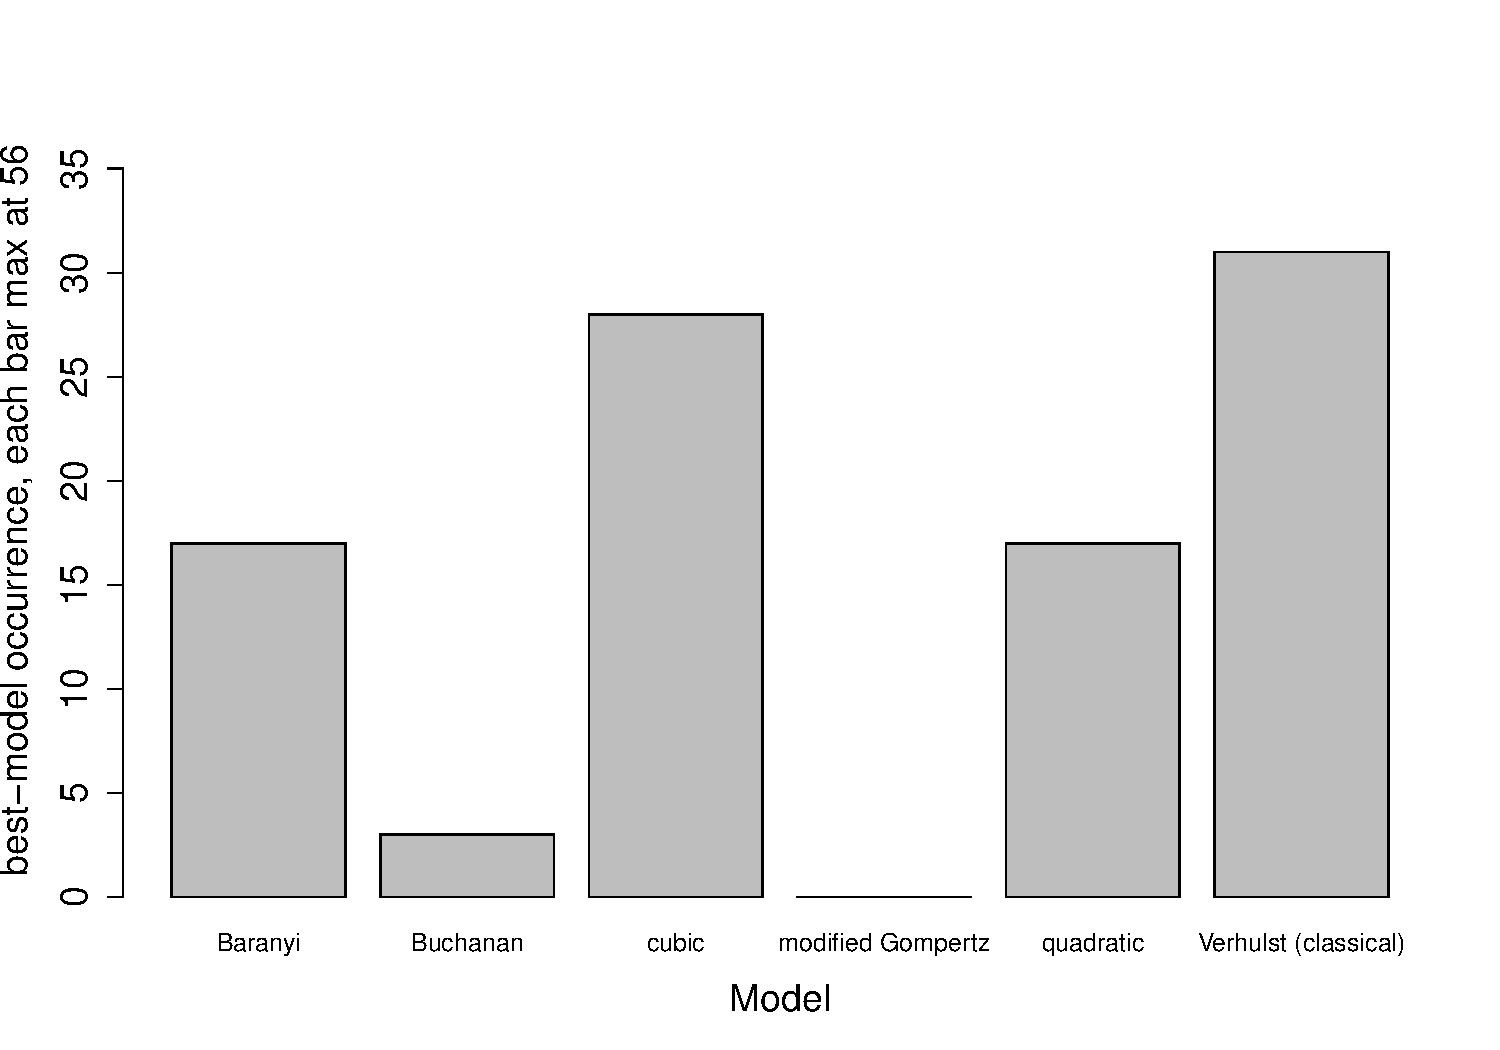
\includegraphics[width=.8\linewidth]{../results/barplot_BestModel.pdf}
		\caption{Barplot showing the number of ``best model" identification under AIC model-selection methods with ``
			%%insert_num_here
			" statistic $X^{2}$ = 
			%% insert_num_here
			, df = 
			%% insert_num_here
			, p = 
			%% insert_num_here
		}\label{barPT}
	\end{figure}
	From Fig.\ref{barPT}, large fluctuations between each model to be described as ``best-fit" were observed.  However the occurrence difference was not statistical significant.  Among the counts, there were 
	%% insert_num_here
	datasets with more than one ``best-fit" models.  \fve\ and \fcu\ were the top two models selected as ``best-fit" for the 
	%% insert_num_here
	 datasets (
	 %%insert_num_here
	  for \fve\ and 
	 %% insert_num_here
	  for \fcu
	 ).  There are 
	 %% insert_num_here
	  datasets calling both ``best-fit" at the same trial.  Between \fba\ and \fqu, the counts were 
	 %%insert_num_here
	  and 
	 %%insert_num_here
	  respectively with 
	 %% insert_num_here
	 datasets calling both models ``best-fit".  The only outstanding performance was from \fgo, which 
	 %% insert_num_here
	  datasets were called it as ``best-fit".
	  
	 \begin{figure}[H]
	 	\centering
	 	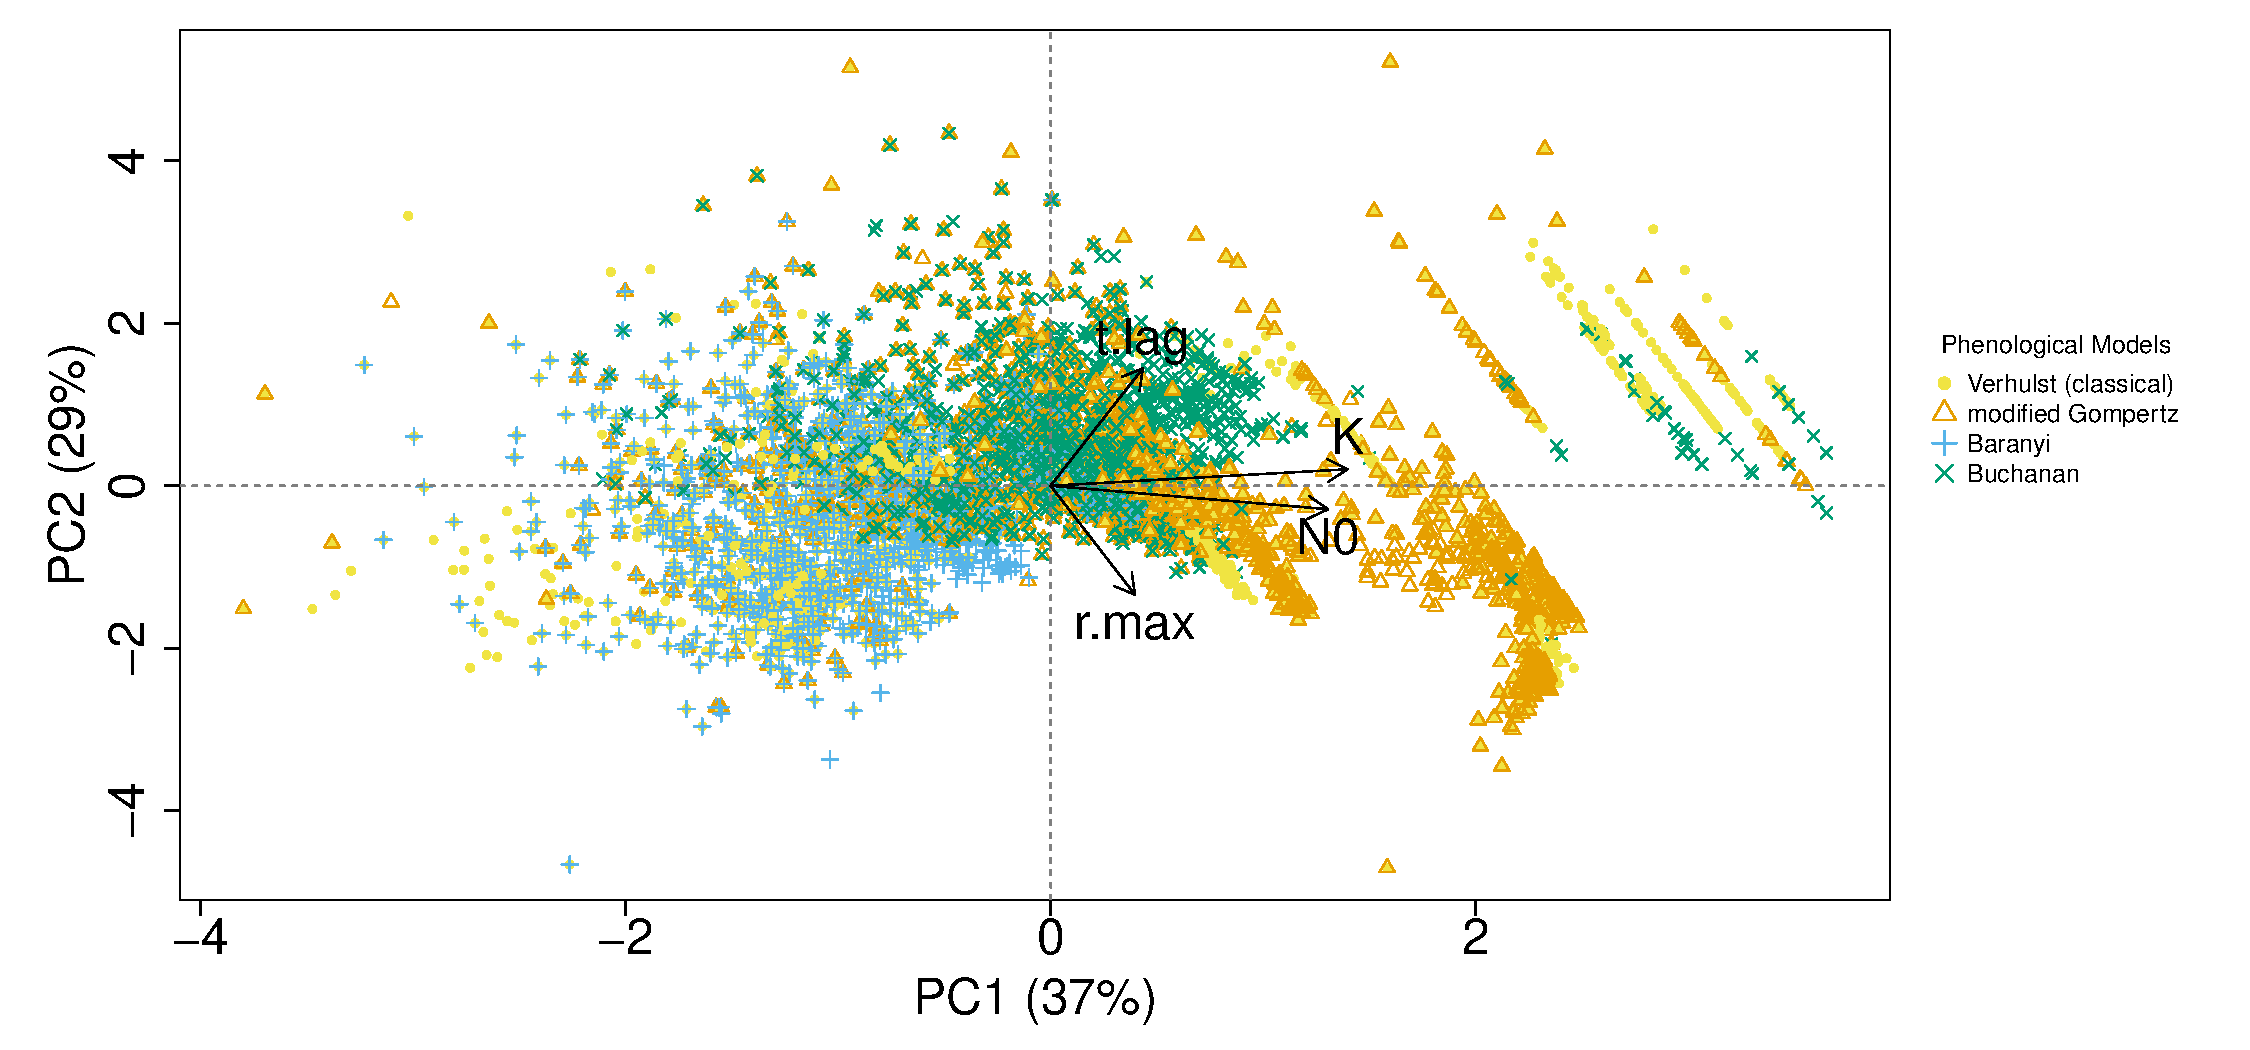
\includegraphics[width=\linewidth]{../results/Log_PCA.pdf}
	 	\caption{Biplot of Principal Component Analysis (PCA) comparing \pms\ using estimated parameter values with ``minimal AIC +2"\autocite{burnham2004multimodel} evaluations.}\label{biptPCA}
	 \end{figure}
 \begin{figure}[H]
 	\centering
 	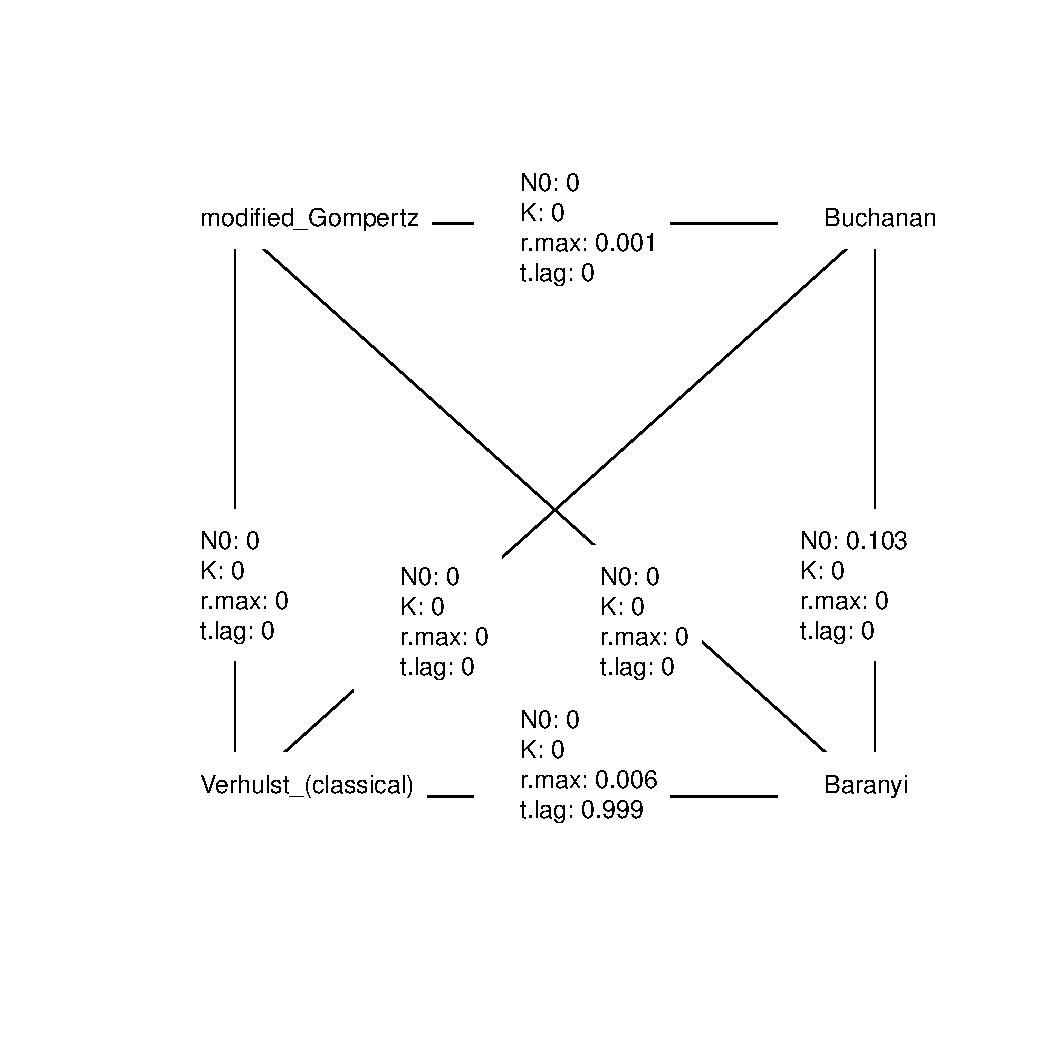
\includegraphics[width=\linewidth]{../results/Log_PCA_kt.pdf}
 	\caption{P-value summary between models on the four parameters under post-hoc Tukey-Dist pairwise comparison from Kruskal-Wallis Test.  Kruskal tests for all four factors were significant (
 		%% insert_num_here
 		: $X^{2}$ =
 		%% insert_num_here
 		, df = 
 		%% insert_num_here
 		, p-value = 
 		%% insert_num_here
 		; 
 		%% insert_num_here
 		: $X^{2}$ =
 		%% insert_num_here
 		, df = 
 		%% insert_num_here
 		, p-value = 
 		%% insert_num_here
 		; 
 		%% insert_num_here
 		: $X^{2}$ =
 		%% insert_num_here
 		, df = 
 		%% insert_num_here
 		, p-value = 
 		%% insert_num_here
 		; 
 		%% insert_num_here
 		: $X^{2}$ =
 		%% insert_num_here
 		, df = 
 		%% insert_num_here
 		, p-value = 
 		%% insert_num_here
 		).}\label{pValDraw}
 \end{figure}
 \begin{figure}[H]
	\centering
	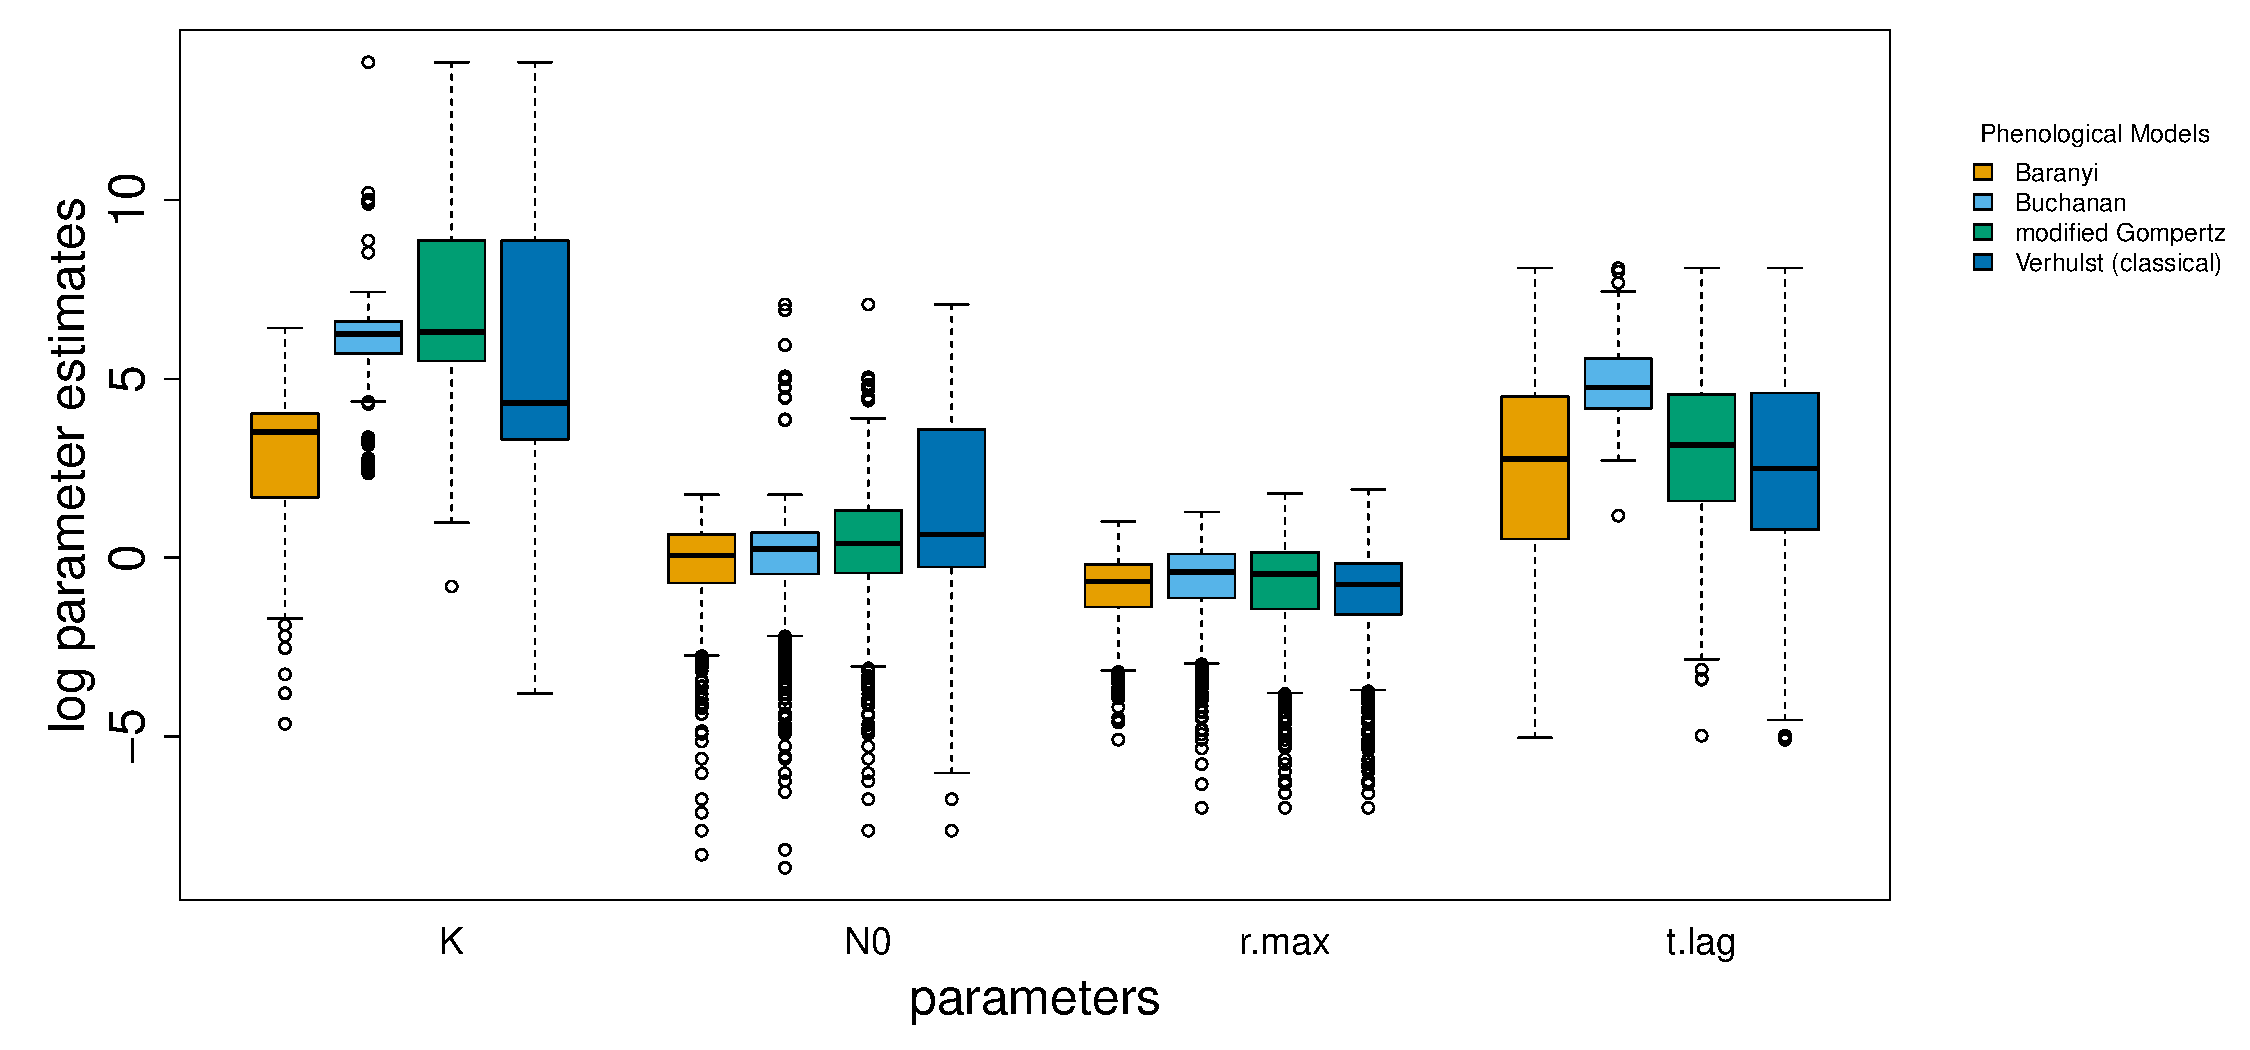
\includegraphics[width=\linewidth]{../results/Log_boxPerFac.pdf}
	\caption{Boxplot of log parameter values grouped by \pms.  Statistical results were summarized in Fig.\ref{pValDraw}}\label{boxFac}
\end{figure}
 In Fig.\ref{biptPCA}, principal component 1 (PC1) was capturing 
 %% insert_num_here
 \% variability.  It was composed approximately by 
 %% insert_num_here
  N0, 
 %%insert_num_here
  K, 
 %% insert_num_here
  r.max and 
 %% insert_num_here
  t.lag.  PC2 was capturing 
  %%insert_num_here
  \% variability.  It was composed approximately by 
 %% insert_num_here
  N0, 
 %%insert_num_here
  K, 
 %% insert_num_here
  r.max and 
 %% insert_num_here
  t.lag.  There were 
 %% insert_num_here
  datasets with \pms\ fitting, although they may not be the ``best-fit" ones.  Datasets 
 %% insert_num_here
  were strictly limited to polynomial-fitting (Fig.\ref{lineOut}).  \fve\ was having the widest neutral coverage across parameter space (Fig.\ref{biptPCA},\ref{boxFac}).  All other three models (\fgo, \fba\ and \fbu) were generally modelling within the \fve\ coverage (Fig.\ref{boxFac}).  \fgo\ was the second widest coverage model but \fve\ was evaluated better if both equations fitted the same dataset (Fig.\ref{barPT}).  More successful trials were towards positive responses for N0, K and r.max.  \fba\ was a specific model more specified in describing datasets with negative responses towards most parameter factors (all except r.max).  \fba\ had the strictest r.max acceptance for successful NLLS modelling (Fig.\ref{boxFac}).  \fbu\ had the narrowest parameter ranges in most parameters (all except r.max, Fig.\ref{boxFac}).  Datasets describable by this model were generally neutral responses towards all four parameters (Fig.\ref{biptPCA}).  In the analysis for individual parameters, the parameter value ranges overlapping between \pms\ (Fig.\ref{boxFac}).  Hence the differences were not observable although most ``differences" were statistically significant (Fig.\ref{pValDraw}).
 \begin{figure}[H]
 	\centering
 	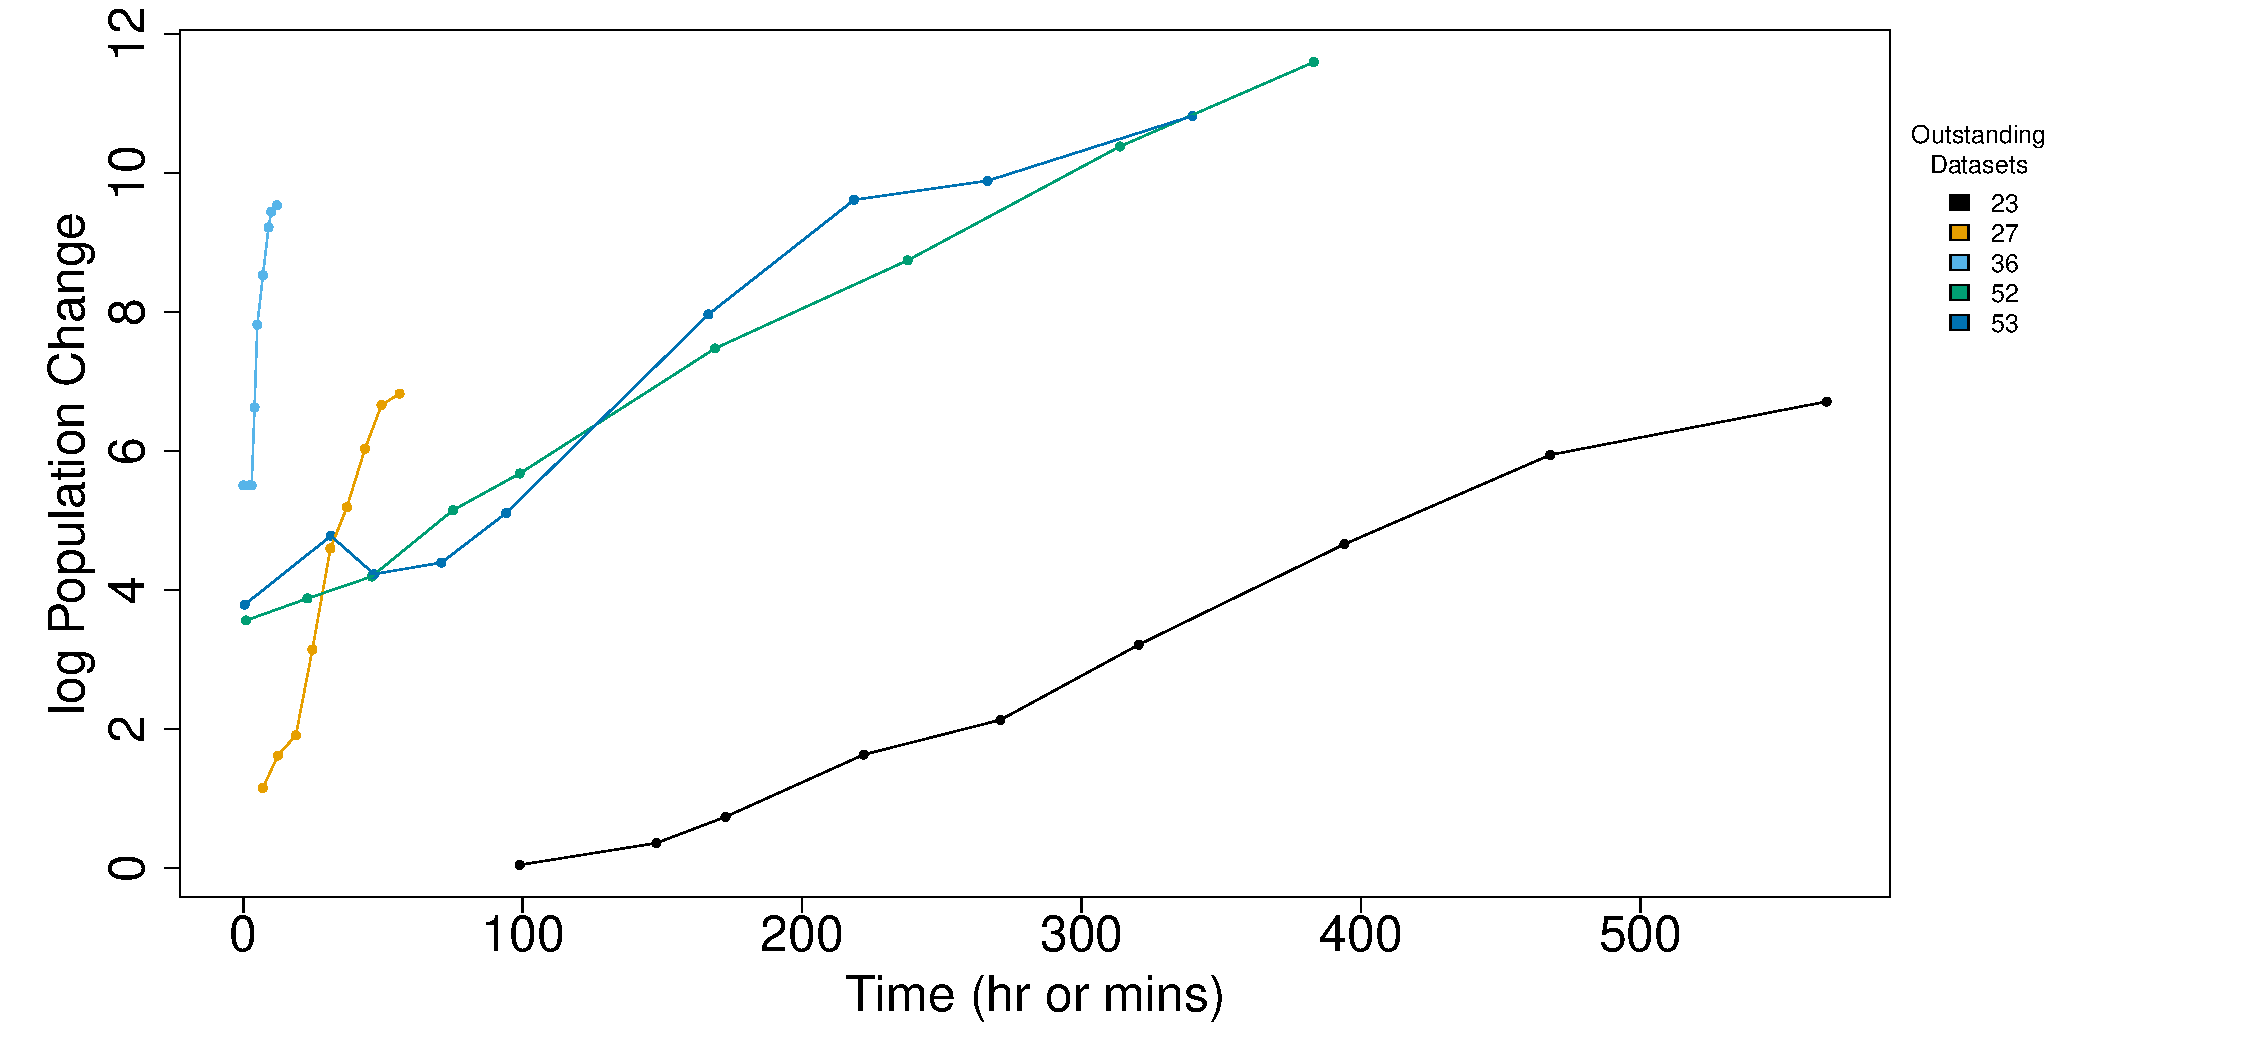
\includegraphics[width=\linewidth]{../results/Log_outstanding.pdf}
 	\caption{Line plot of datasets restricted to polynomial fits. Dataset details could be found in Table \ref{table:source}}\label{lineOut}
 \end{figure}

	Using Kruskal test, microbial clade was significantly correlated with the experimental growth media ($X^{2}$ =
	%% insert_num_here
	, df = 
	%% insert_num_here
	, p-value = 
	%% insert_num_here
	).  Hence downstream analyses had taken both factors as a combined independent variable.  Based on the combined factor, Kruskal test were done using dependent variable of ``optimal model type" ($X^{2}$ =
	%% insert_num_here
	, df = 
	%% insert_num_here
	, p-value = 
	%% insert_num_here
	), ``N0" ($X^{2}$ =
	%% insert_num_here
	, df = 
	%% insert_num_here
	, p-value = 
	%% insert_num_here
	), ``K" ($X^{2}$ =
	%% insert_num_here
	, df = 
	%% insert_num_here
	, p-value = 
	%% insert_num_here
	), ``r.max" ($X^{2}$ =
	%% insert_num_here
	, df = 
	%% insert_num_here
	, p-value = 
	%% insert_num_here
	) and ``t.lag" ($X^{2}$ =
	%% insert_num_here
	, df = 
	%% insert_num_here
	, p-value = 
	%% insert_num_here
	).  Among the parameters, r.max was the only factor without significance.  However posthoc Nemenyi test showed that none of the factor pairs (out of 
	%% insert_num_here
	pairs) were statistically significant although the Kruskal test showed otherwise.
	
	\section*{Discussion}
	%% AIC vs BIC <https://www.methodology.psu.edu/resources/AIC-vs-BIC/>
	%% AIC <https://en.wikipedia.org/wiki/Akaike_information_criterion#Comparison_with_BIC>
	%% BIC <https://en.wikipedia.org/wiki/Bayesian_information_criterion>
	%Model fitness to real data and simplistic mathematics were favoured by both AIC\autocite{johnson2004model,akaike1998information,burnhamdr} and BIC\autocite{johnson2004model,turchin2003complex}.  Apart from that, BIC also takes account of sample size effect\autocite{johnson2004model,turchin2003complex}.\\
	%comparisons in different fields\autocite{kuha2004aic,aho2014model,yang2005can,vrieze2012model,wang2006comparison,acquah2010comparison}\\
	
	AIC is the most suitable approach (compare with BIC and R$^2$) for model evaluation within and between models in this project because AIC 1. is accurate with small sample size\autocite{acquah2010comparison,kuha2004aic} and sparse data\autocite{kuha2004aic}; 2. does not assume a ``true model" was under examination\autocite{aho2014model,vrieze2012model,yang2005can}; and 3. take number of parameters into evaluation consideration\autocite{johnson2004model}.  Also none of the \pms\ used are ``nested"\autocite{wang2006comparison}, leaving AIC as the only appropriate model-selection method.
	
	\Pms\ were not always better than polynomials.  Since experimental data is highly variable, some may not fit assumptions of these models (Fig.\ref{lineOut}).  Even among the fitted ones, \pms\ are not statistically better than polynomials (Fig.\ref{barPT}).  Reasons for data unable to be fitted by a ecological model can be due to different reasons within three categories: unfit model, unfit data and assumptions in model not met.  The chance for having ``unfit model" is small because there are multiple fits in other datasets summarized in Fig.\ref{biptPCA} for each \pms.  Some datasets are clearly ``unfit data" (e.g. dataset 36, 52 and 53; Fig.\ref{lineOut}).  They share similar properties: few record points, data line-up in a fairly linear manner and not much curvatures are observed.  These are not typical logistic growth curves.  The reasons generating these data can be due to the insufficient experiment time (hence no carrying capacity plateau has observed), improper culture-handling before the start of experiments (hence no initial \pps\ recorded as the microbial clade has already adapted to the experiment environment) and/or coarse data record intervals (hence too many population fluctuation features missed within recording intervals).  One or more reasons can potentially related to the data in Fig.\ref{lineOut}.  The other two datasets (i.e. datasets 23 and 27) may fall into the third category.  By observations, these two datasets can potentially be described by \pms.  However the reasons for unsuccessful NLLS modelling can be due to the small data sizes.  N0 and K values can be extrapolated but not calculated.  There are only one data point on each end of the line indicating a curve direction change.  As \pms\ need multiple data records to support N0 and K values as parameters, these two datasets can probably only satisfy the r.max requirement.  Hence these two datasets are also considered not \pml-friendly.
	
	Between \pms, some of them may be highly specific (e.g. \fba\ and \fbu) or general (e.g. \fve\ and \fgo).  Although PCA result shows significant separation of model properties (Fig.\ref{biptPCA},\ref{pValDraw},\ref{boxFac}), these differences are not observable in the data (Fig.\ref{boxFac}).  The clustering of NLLS parameter estimates is also not having defined boundaries (Fig.\ref{biptPCA}), increasing the difficulty of choosing the most appropriate \pml\ for a newly-generated microbial \pps\ dataset.  Due to the different \pml\ properties towards their own parameters (Fig.\ref{biptPCA}), the PCA graph can be a reference for determining the best \pml\ on those new data in the future.  However Fig.\ref{biptPCA} can only be used literally when the experimental temperature, substrate and population unit of the microbial clades all fall within the categories or ranges listed in Table \ref{table:source}.  If not, the same methodology can be used with suitable published data to generate the PCA result for reference.  Generally speaking, \fve\ will be sufficient to explain most behaviours of the population.  \fgo\ can be used when authors want to incorporate t.lag into description, although this factor may be redundant (Fig.\ref{barPT}).  Using Fig.\ref{biptPCA} as reference, one can pinpoint the data response to the parameters and refine their model-of-choice to a more specific one if necessary.
	
	On biological side, the analyses show that microbial identity and the growth media are statistically significant as expected.  Hence they should be analysed as one factor because there is no method to isolate one from the other.  Yet this combined factor does not have statistically significant indicative number on their initial, climax population size, their maximum growth rate nor the lag phase duration.
	
	\section*{Conclusion}
	Published \pms\ were data-specific, which none of them were found significantly performing better than the others.  Although most of the parameter values are significantly different between models, their ranges are superimposing with one another.  \Pms\ correlate with parameters differently, but the correlations are unobservable through plotting a log-linear logistic growth curve.  There were assumptions embedded within \pms\ which have limited its ability to describe data without a distinct sigmoid shape.  Biologically, microbial identity has no indication on how they grow in laboratory conditions.  Hence these parameters, if needed for researches, have to be measured case-by-case.
	
	\section*{Code and Data Availability}
	All \href{https://github.com/ph-u/CMEECourseWork_pmH/tree/master/MiniProject/code}{scripts} and \href{https://github.com/ph-u/CMEECourseWork_pmH/tree/master/MiniProject/data}{data} used for this report were publicity available at GitHub.
	\nocite{*}\printbibliography
	
	\section*{Appendix}
\begin{table}[H]
		\caption{Table showing dataset id details in this project.}\label{table:source}
\end{table}
\begin{small}
	\begin{longtable}{l|llllll}
		id&T$^{o}$C&clade&substrate&replicate&Source&Pop unit\\\hline
		%% insert_num_here
	\end{longtable}
\end{small}
``Source" column publication key:\\
\begin{longtable}{p{.05\linewidth}|p{.9\linewidth}}
	%% insert_num_here
	%% insert_num_here
	%% insert_num_here
	%% insert_num_here
	%% insert_num_here
	%% insert_num_here
	%% insert_num_here
	%% insert_num_here
	%% insert_num_here
	%% insert_num_here
\end{longtable}

\end{document}
